\paragraph{}

\section{Image Thresholding}
\paragraph{Introduction}
Thresholding is a process of creating binary image from a grayscale one.\cite{digital-image-processing} It is the simplest form of segmentation (separating image into regions). It uses the simplest property that pixels in a region can share - the intensity. Hence thresholding is a natural way of separating light and dark regions of the image. In simple words, all pixels with intensity value below some threshold are being assigned zero and all pixels with intensity above this threshold one. Pixels that are equal the threshold value are treated either as zero or one but the behaviour needs to be consistent. 

\paragraph{}
Let $f(x, y)$ be the gray level of pixel $(x, y)$ and $T$ be the threshold value, then the thresholded image $g(x, y)$ is defined as:

\begin{equation}
	g(x, y) = \begin{cases}
		1 & \text{if $f(x, y) >= T$}\\
		0 & \text{otherwise}
	\end{cases}
\end{equation}

\paragraph{}
Every point $(x, y)$ for which $f(x, y) >= T$ is then called an \textit{object point}, whereas all the other ones are said to be \textit{background points}.

\paragraph{Problems with thresholding}
The most significant issue with thresholding is the fact that only the intensity is considered and no relationship between pixels is. This can lead to the inclusion of external pixels that are not part of the original region. Similarly, isolated pixels can be lost from a region. The presence of noise in the image can easily worsen the outcome, because pixels intensity may not represent the normal intensity in the region. The usage of thresholding is often based on experimentation and small adjustments. Still, a large portion of a region may be lost or the area may be extended with extraneous background pixels (especially when shadows of objects are presents - which causes them to be included as part of dark object on a light background). One of the flaws of global image thresholding is also the fact that it is not particularly effective when changes in illumination occur in the image. This drawback can partially be mitigated by determining thresholds locally, so instead of a single global threshold value, the threshold itself can actually vary across different parts of the image.

\paragraph{}
Figures \ref{fig:threshold_variants} and \ref{fig:threshold_examples} present the various threshold variants available in OpenCV.

\begin{figure}[H]
	\centering
	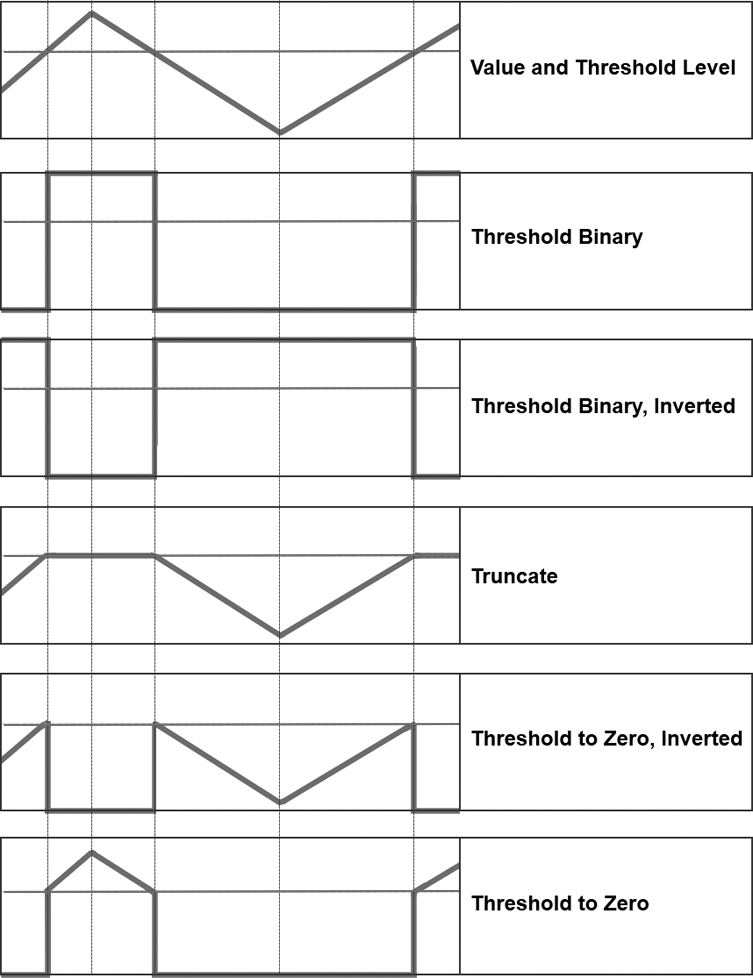
\includegraphics[width=\textwidth]{images/thresholds}
	\caption{Threshold variants in OpenCV}
	\source{\cite{learning-opencv-3}, Figure 10-4}
	\label{fig:threshold_variants}
\end{figure}

\begin{figure}
	\centering
	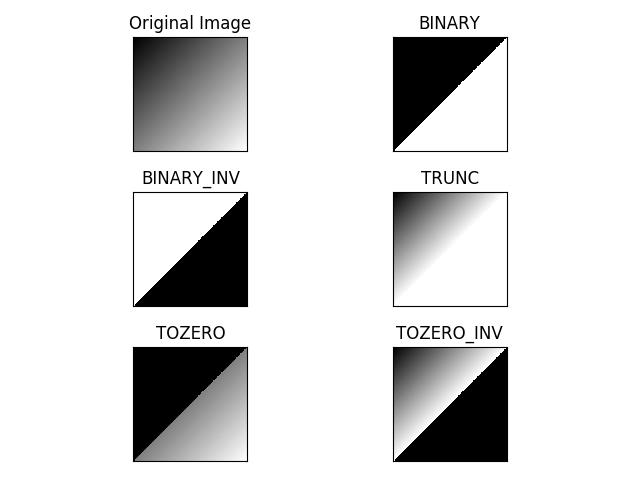
\includegraphics[width=\textwidth]{images/thresholds_example}
	\caption{Example usage of thresholds in OpenCV}
	\label{fig:threshold_examples}
\end{figure}

\section{Image Filtering}
\paragraph{Introduction}
Filtering is a technique for modifying or enhancing an image. It is used either to emphasize some features of the image or to remove some other. Images can be filtered with various low-pass filters (LPF) or high-pass filters (HPF). HPFs are useful for finding edges in the images whereas LPFs are used to remove noise and for image blurring.

\paragraph{Correlation and convolution}\cite{correlation-convolution}
This are basic operations that can be applied in order to extract information from an image. In a sense they are the simplest operations that can be performed but, nevertheless, extremely powerful and useful. Due to their simplicity they are also well understood, easy implementable and efficiently computable. Both of these operations fullfill two features:
\begin{itemize}
	\item Linearity
	\item Shift-invariance
\end{itemize}
Let us now look at correlation in 2D. Given a square filter with odd number of elements represented by a $(2N + 1)$ x $(2N + 1)$ matrix $F$ and the image matrix $I$, the results of correlation can be computed by aligning the center of the filter with a pixel. Overlapping values are then multiplied together and summed up to make the result corresponding to that given pixel. It can be written as
\begin{equation}
	(F \otimes I)(x, y) = \sum_{i = -N}^{N}\sum_{j = -N}^{N}F(i, j)I(x + i, y + j)
\end{equation}
Convolution is very similar to correlation, but the filter is flipped both horizontally and vertically beforehand. 
\begin{equation}
	(F \star I)(x, y) = \sum_{i = -N}^{N}\sum_{j = -N}^{N}F(i, j)I(x - i, y - j)
\end{equation}

\paragraph{}
Let us now see a simple example presenting difference between correlation and convolution. Equation \ref{eq:correlation} shows a very basic example of correlation.
\begin{equation}
\begin{bmatrix}
    0 & 0 & 0 & 0 & 0 & 0 & 0 \\
    0 & 0 & 0 & 0 & 0 & 0 & 0 \\
    0 & 0 & 0 & 0 & 0 & 0 & 0 \\
    0 & 0 & 0 & 1 & 0 & 0 & 0 \\
    0 & 0 & 0 & 0 & 0 & 0 & 0 \\
    0 & 0 & 0 & 0 & 0 & 0 & 0 \\
    0 & 0 & 0 & 0 & 0 & 0 & 0 \\            
\end{bmatrix}
\otimes
\begin{bmatrix}
    a & b & c \\
    d & e & f \\
    g & h & i
\end{bmatrix}
=
\begin{bmatrix}
    0 & 0 & 0 & 0 & 0 & 0 & 0 \\
    0 & 0 & 0 & 0 & 0 & 0 & 0 \\
    0 & 0 & i & h & g & 0 & 0 \\
    0 & 0 & f & e & d & 0 & 0 \\
    0 & 0 & c & b & a & 0 & 0 \\
    0 & 0 & 0 & 0 & 0 & 0 & 0 \\
    0 & 0 & 0 & 0 & 0 & 0 & 0 \\            
\end{bmatrix}
\label{eq:correlation}
\end{equation}

\paragraph{}
Equation \ref{eq:convolution}, on the other hand, presents a convolution. We can see that it is indeed equivalent to a correlation with a flipped filter.

\begin{equation}
\begin{array}{l}
\begin{bmatrix}
    0 & 0 & 0 & 0 & 0 & 0 & 0 \\
    0 & 0 & 0 & 0 & 0 & 0 & 0 \\
    0 & 0 & 0 & 0 & 0 & 0 & 0 \\
    0 & 0 & 0 & 1 & 0 & 0 & 0 \\
    0 & 0 & 0 & 0 & 0 & 0 & 0 \\
    0 & 0 & 0 & 0 & 0 & 0 & 0 \\
    0 & 0 & 0 & 0 & 0 & 0 & 0 \\            
\end{bmatrix}
\star
\begin{bmatrix}
    a & b & c \\
    d & e & f \\
    g & h & i
\end{bmatrix}
= \\ \\
=
\begin{bmatrix}
    0 & 0 & 0 & 0 & 0 & 0 & 0 \\
    0 & 0 & 0 & 0 & 0 & 0 & 0 \\
    0 & 0 & 0 & 0 & 0 & 0 & 0 \\
    0 & 0 & 0 & 1 & 0 & 0 & 0 \\
    0 & 0 & 0 & 0 & 0 & 0 & 0 \\
    0 & 0 & 0 & 0 & 0 & 0 & 0 \\
    0 & 0 & 0 & 0 & 0 & 0 & 0 \\            
\end{bmatrix}
\otimes
\begin{bmatrix}
    i & h & g \\
    f & e & d \\
    c & b & a
\end{bmatrix}
=
\begin{bmatrix}
    0 & 0 & 0 & 0 & 0 & 0 & 0 \\
    0 & 0 & 0 & 0 & 0 & 0 & 0 \\
    0 & 0 & a & b & c & 0 & 0 \\
    0 & 0 & d & e & f & 0 & 0 \\
    0 & 0 & g & h & i & 0 & 0 \\
    0 & 0 & 0 & 0 & 0 & 0 & 0 \\
    0 & 0 & 0 & 0 & 0 & 0 & 0 \\            
\end{bmatrix}
\end{array}
\label{eq:convolution}
\end{equation}

\paragraph{}
The key distinction before the two operations is the associative property of convolution:
\begin{equation}
	\forall F, G - filters \quad \forall I - image: F \star (G \star I) = (F \star G) \star I
\end{equation}
This property is useful when there is need to convolve image with multiple filters. It is computationally faster to precompute the final filter as convolution of original filters and apply just one convolution to the input image. Convolutions are used for image processing operations such as smoothing whereas correlations are useful for matching templates.
One final notice, that for symmetrical filters convolution and correlation are identical.

\paragraph{Image blurring}
To achieve smoothing effect, the image is convolved with a LPF kernel. This particular type of filtering removes high frequency content from the image (for example noise). Unfortunately, edges also can be blurred a bit while applying this operation, although there are also smoothing filters that prevent edges from being blurred. The OpenCV library provides user with various filters amongst which the most popular ones are:
\begin{itemize}
	\item Averaging - it takes the average of all the pixels under kernel area
	\item Gaussian - instead of box filter, a Gaussian kernel is used
	\item Median - in this case the median value of all the pixels under kernel area is used
	\item Bilateral - slower compared to other filters, but it keeps edges sharp
\end{itemize}

\section{Morphological Transformations}
\paragraph{}
Morphological transformations are operations based on the image shape. Two inputs are needed to perform such a transformation, one being the original image whereas the other, called kernel, decides the nature of operation. It is performed on binary images, with black background (having value 0) and white foreground (having value 1). Two most basic ones are erosion and dilation which will now be presented.

\paragraph{}
\textbf{Erosion} - erodes away the boundaries of the foreground object. It is performed by sliding the kernel over the image. For each pixel the following equation is applied.

\begin{equation}
	Erosion(pixel, kernel) = \begin{cases}
		1 & \text{if all the pixels under $kernel$ are 1}\\
		0 & \text{otherwise}
	\end{cases}
\end{equation}

When the output of erosion is 0, the pixel is said to be eroded.

\paragraph{}
\textbf{Dilation} - on the other hand, it is the opposite of erosion. 

\begin{equation}
	Erosion(pixel, kernel) = \begin{cases}
		1 & \text{if at least one pixel under $kernel$ is 1}\\
		0 & \text{otherwise}
	\end{cases}
\end{equation}

\paragraph{}
Figure \ref{fig:morphological_examples} shows both erosion and dilation applied to some simple image. It also presents one more morphological transformation, which is just a combination of both of them, \textbf{gradient} - a difference between dilation and erosion of an image.

\begin{figure}[H]
	\centering
	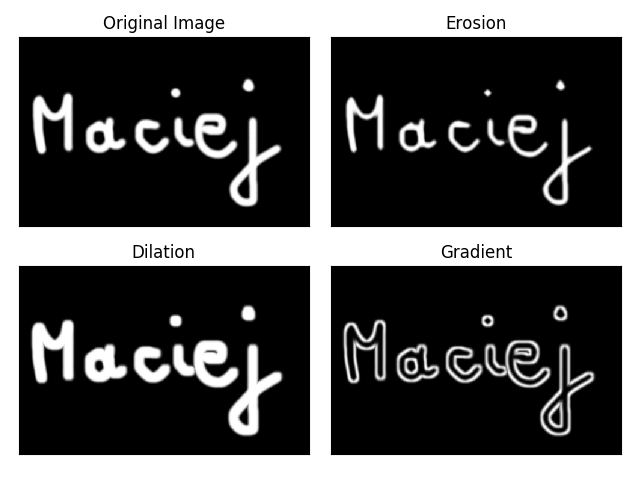
\includegraphics[width=\textwidth]{images/morphological}
	\caption{Example of morphological transformations}
	\label{fig:morphological_examples}
\end{figure}

\section{Finding Contours}
\paragraph{}
A contour is a list of points that represent, in one way or another, a curve in an image.\cite{learning-opencv-3} They come in handy for analysing the shape of an object, for its detection and for recognition. For better results it is good to use binary images, so the process of contours finding should be applied after thresholding or edge detecting.

\paragraph{}
Figure \ref{fig:preprocessing} shows what the process of finding contours can lead to - detecting the shape of an object.

\section{Edge Detection}
\subsection{Derivatives and edges}
An edge is a place of a sudden discontinuity in an image, which can arise from surface normal, surface color, depth, illumination, or other discontinuities. This rapid change in the image intensity function can be observed in places where the first derivative of this function has local extrema (see Figure \ref{fig:edge-detection}).\cite{edge-detection}
\begin{figure}[H]
     \centering
     \subfloat[Original Image]{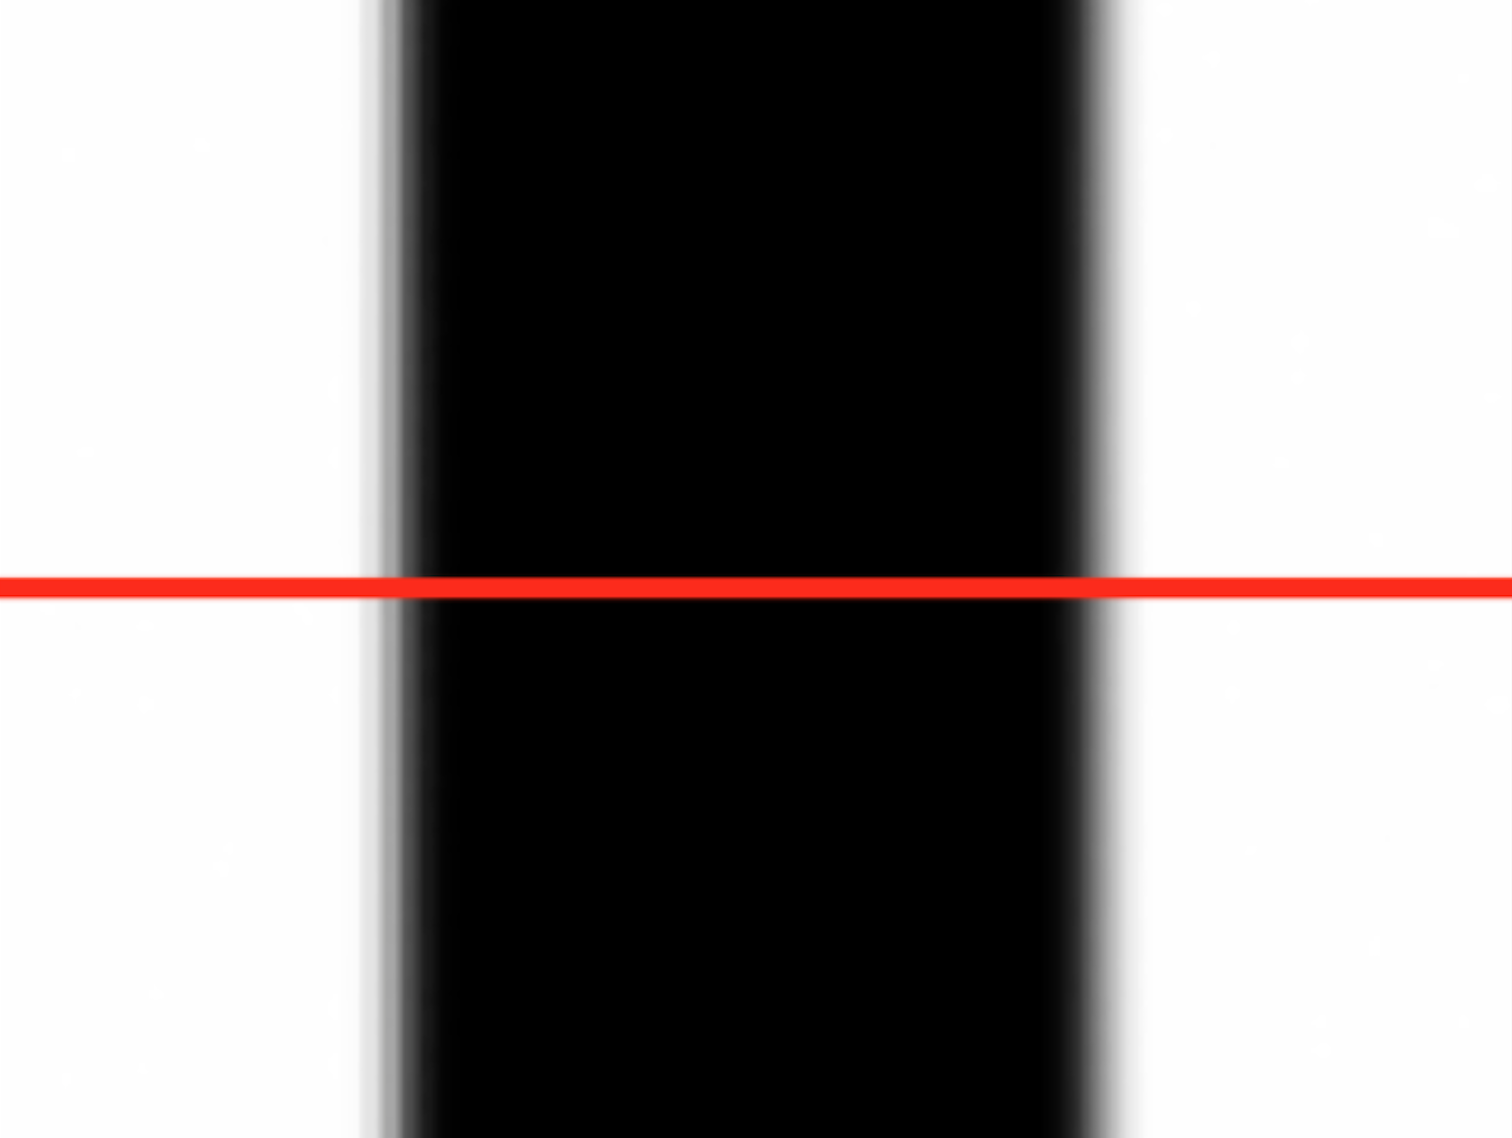
\includegraphics[width=0.5\textwidth]{images/edge_image}}
     \vfill
     \subfloat[Intensity along the specified line]{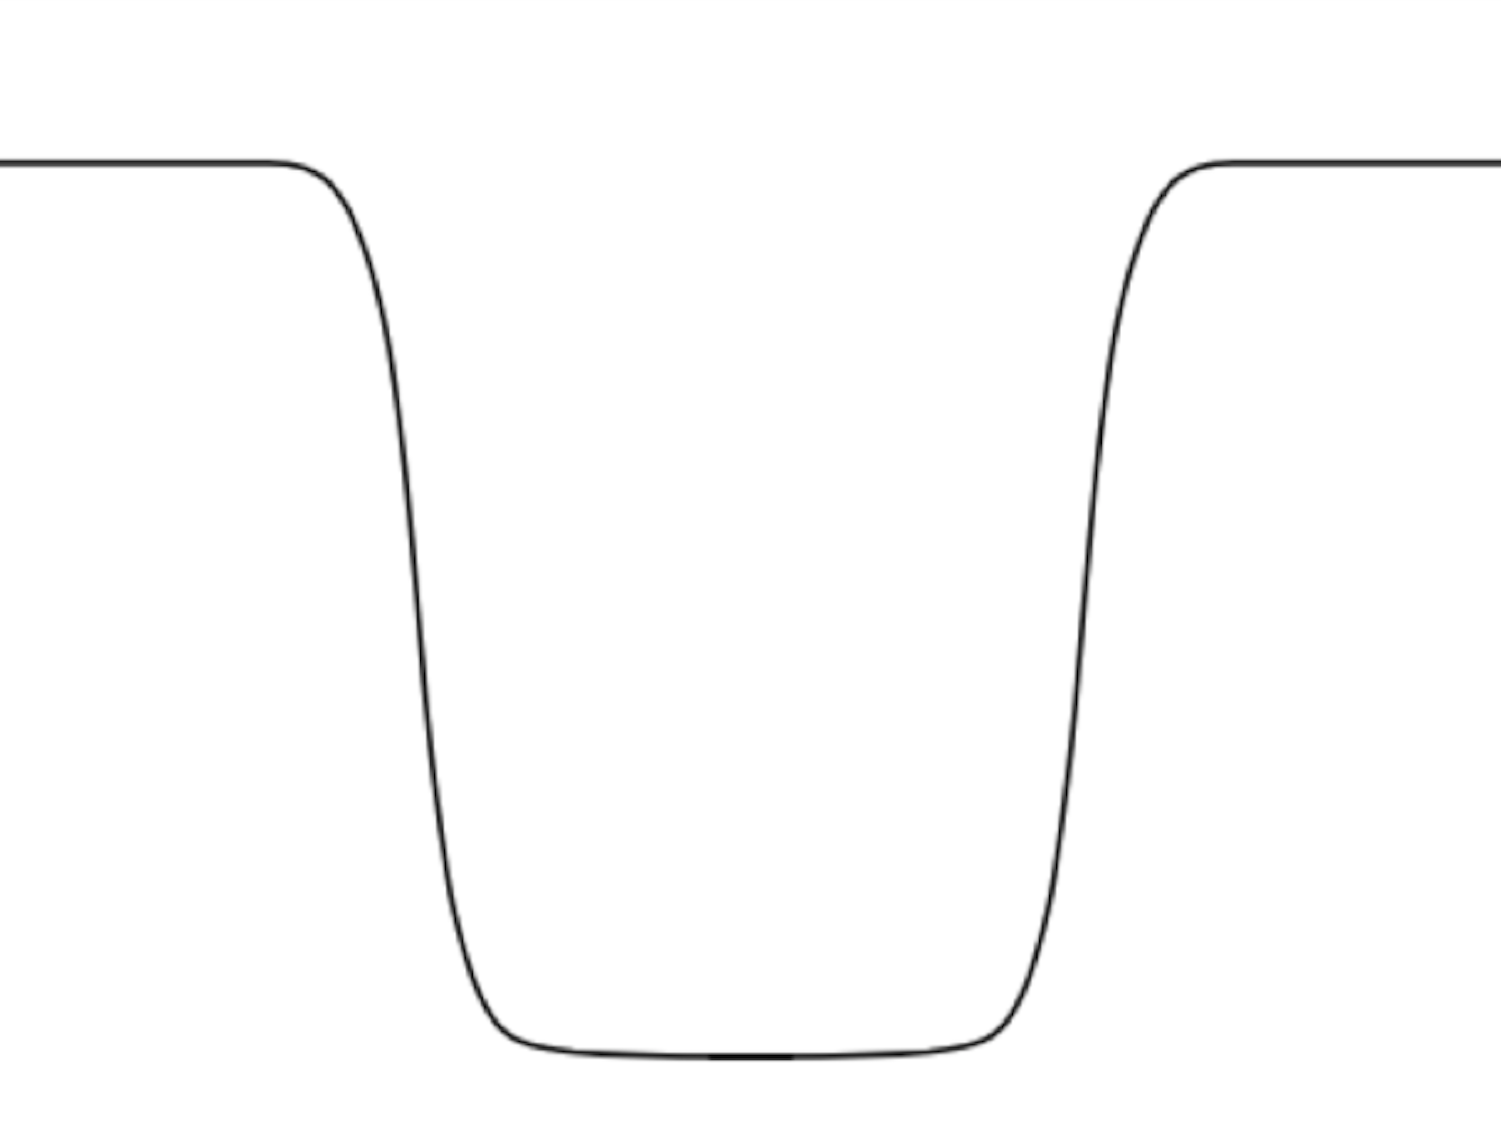
\includegraphics[width=0.5\textwidth]{images/edge_intensity_function}}
     \vfill
     \subfloat[Derivative of the intensity function]{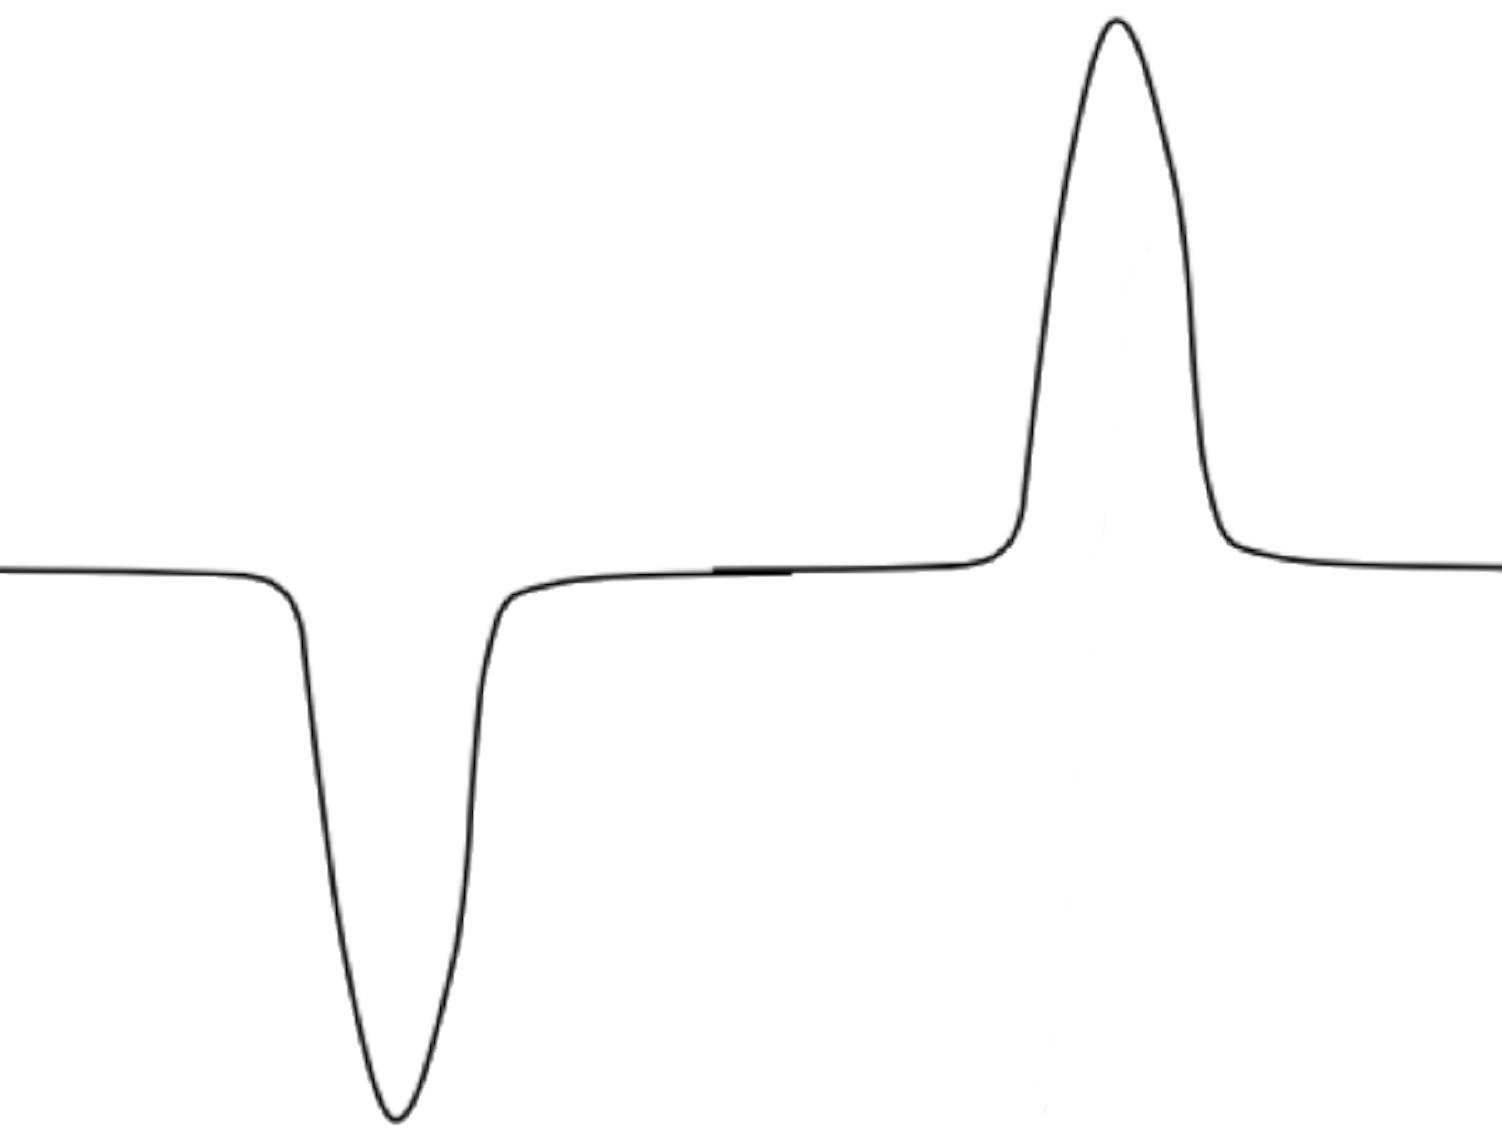
\includegraphics[width=0.5\textwidth]{images/edge_first_derivative}}
     \caption{Edge detection}
     \label{fig:edge-detection}
     \source{\cite{lazebnik-edge}, Slide 4}
\end{figure}

\subsection{Image gradient}
The gradient points in the direction of most rapid increase in intensity and can be represented as:
\begin{equation}
	\nabla f = [\frac{\partial f}{\partial x}, \frac{\partial f}{\partial y}]
\end{equation}
The direction of the gradient is given by:
\begin{equation}
	\theta = tan^{-1}(\frac{\partial f}{\partial y} / \frac{\partial f}{\partial x})
\end{equation}
And, finally, the \textit{amount of change} is given by the gradient magnitude:
\begin{equation}
	\parallel \nabla f \parallel = \sqrt{(\frac{\partial f}{\partial x})^2 + (\frac{\partial f}{\partial y})^2}
\end{equation}
Remember, that for 2D function partial derivative is defined as:
\begin{equation}
	\frac{\partial f(x,y)}{\partial x} = \lim_{\epsilon \to 0} \frac{f(x + \epsilon, y) - f(x, y)}{\epsilon}
\end{equation}
But for discrete data this definition needs to be approximated using finite differences:
\begin{equation}
	\frac{\partial f(x,y)}{\partial x} \approx \frac{f(x + 1, y) - f(x, y)}{1} \approx f(x + 1, y) - f(x, y)
\end{equation}
In order to obtain an operator (a kernel) that implements the definition of the discrete gradient, we end up with averaging "left" and "right" derivative and obtain the kernel:
\[
\frac{1}{2}
(\begin{bmatrix}
    0 & 0 & 0 \\
    -1 & 1 & 0 \\
    0 & 0 & 0
\end{bmatrix}
+
\begin{bmatrix}
    0 & 0 & 0 \\
    0 & -1 & 1 \\
    0 & 0 & 0
\end{bmatrix})
=
\begin{bmatrix}
    0 & 0 & 0 \\
    \frac{-1}{2} & 0 & \frac{1}{2} \\
    0 & 0 & 0
\end{bmatrix}
\]

{\renewcommand{\arraystretch}{2}
\begin{table}[H]
	\centering
	\begin{tabular}{ccc}
		 & \textbf{X} & \textbf{Y} \\
		\hline
		\\
		\textbf{Sobel} & $\begin{bmatrix} -1 & 0 & 1 \\ -2 & 0 & 2 \\ -1 & 0 & 1 \end{bmatrix}$ & $\begin{bmatrix} 1 & 2 & 1 \\ 0 & 0 & 0 \\ -1 & -2 & -1\end{bmatrix}$ \\
		\\
		\hline
		\\
		\textbf{Prewitt} & $\begin{bmatrix} -1 & 0 & 1 \\ -1 & 0 & 1 \\ -1 & 0 & 1 \end{bmatrix}$ & $\begin{bmatrix} 1 & 1 & 1 \\ 0 & 0 & 0 \\ -1 & -1 & -1 \end{bmatrix}$ \\
		\\
		\hline
		\\
		\textbf{Roberts} & $\begin{bmatrix} 1 & 0 \\ 0 & -1 \end{bmatrix}$ & $\begin{bmatrix} 0 & 1 \\ -1 & 0 \end{bmatrix}$ \\
		\\
		\hline
	\end{tabular}
	\caption{Some of the well-known gradient kernels}
\end{table}
}
In the real world the intensity function is affected by noise and may look like in Figure \ref{fig:noise_intensity_function}
\begin{figure}[H]
	\centering
	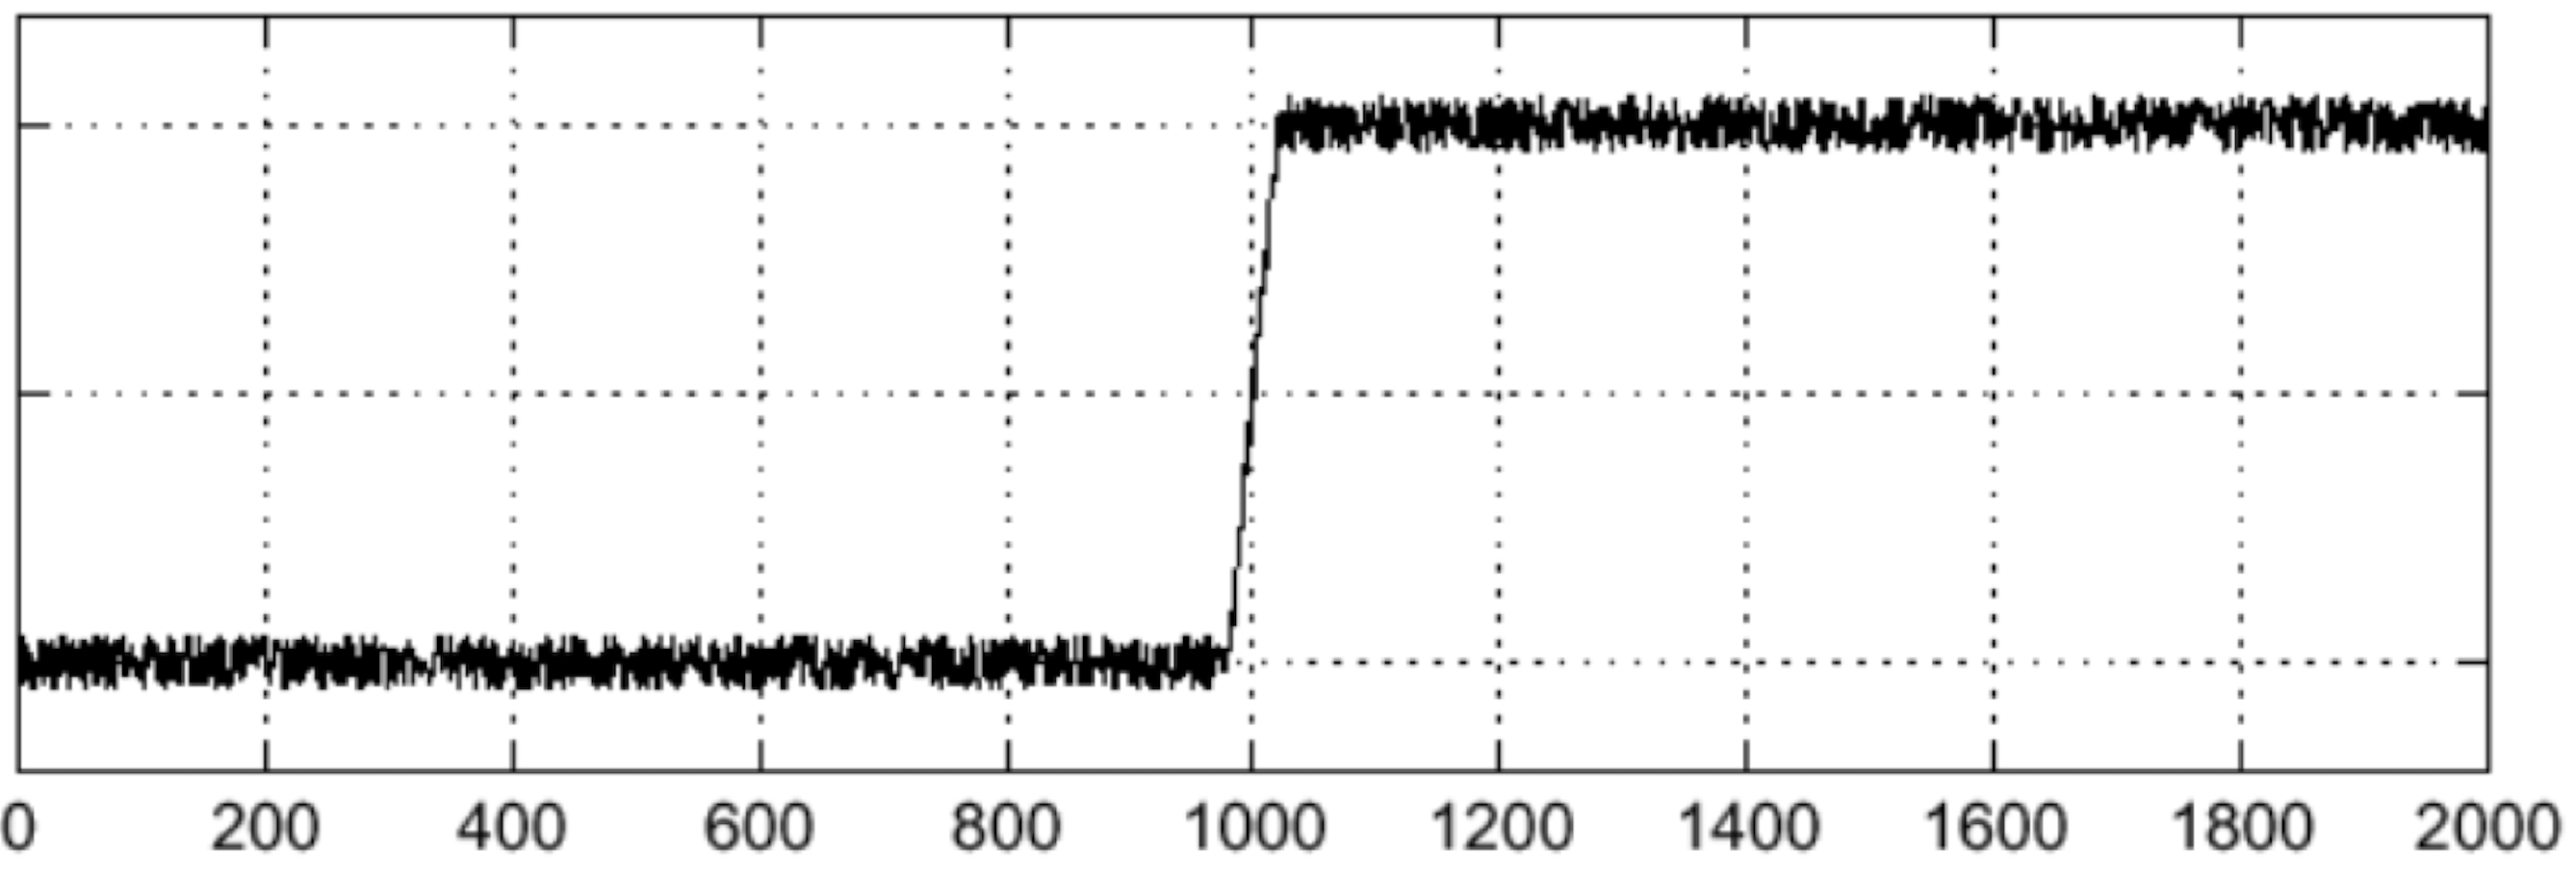
\includegraphics[width=\textwidth]{images/noise_intensity_function}
	\caption{Intensity function affected by noise}
	\source{\cite{lazebnik-edge}, Slide 10}
	\label{fig:noise_intensity_function}
\end{figure}
This can cause the result of applying the derivative operator to be unable to tell where the edge might be (see Figure \ref{fig:noise_derivative})
\begin{figure}[H]
	\centering
	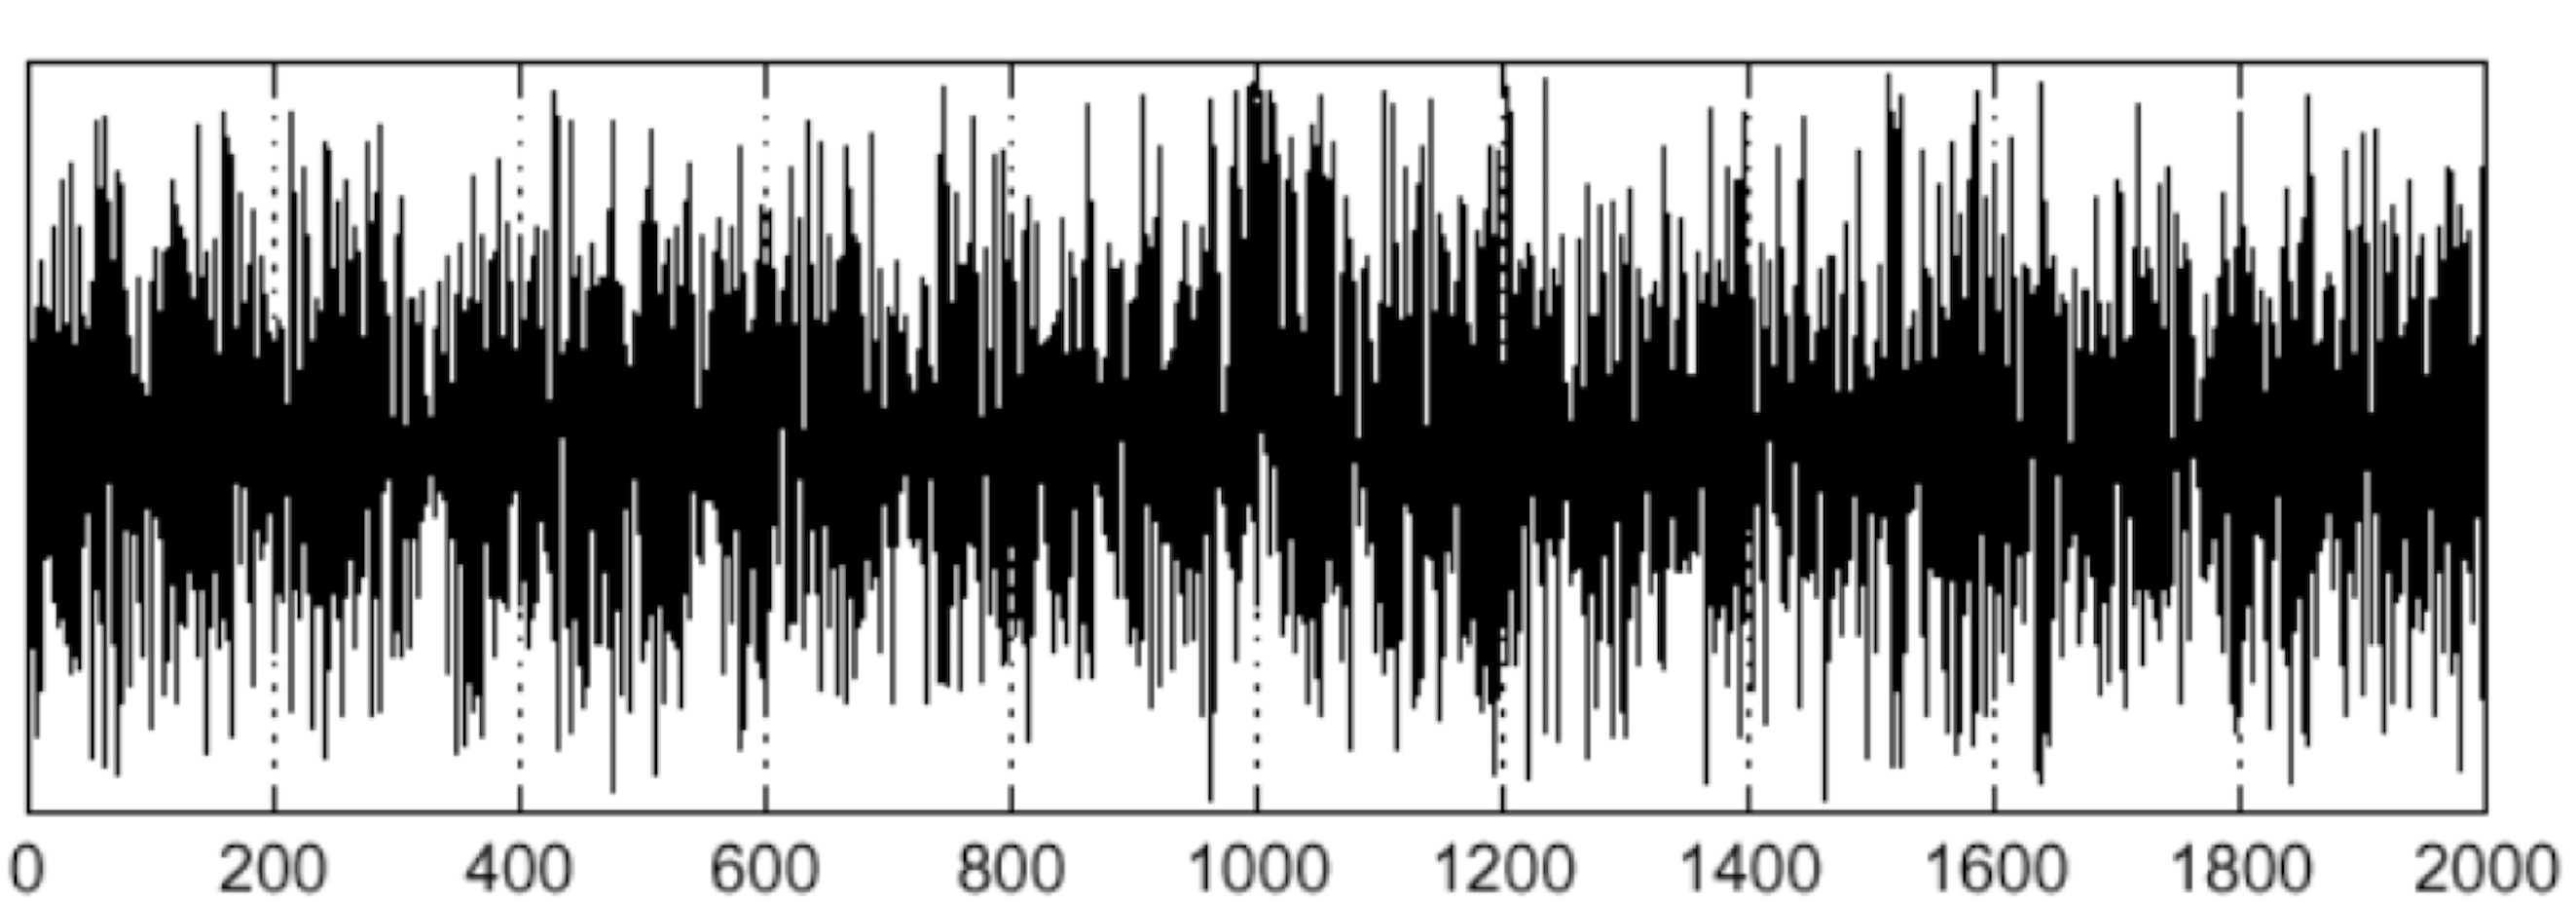
\includegraphics[width=\textwidth]{images/noise_derivative}
	\caption{Derivative of the intensity function affected by noise}
	\source{\cite{lazebnik-edge}, Slide 10}
	\label{fig:noise_derivative}
\end{figure}
\begin{figure}[H]
	\centering
	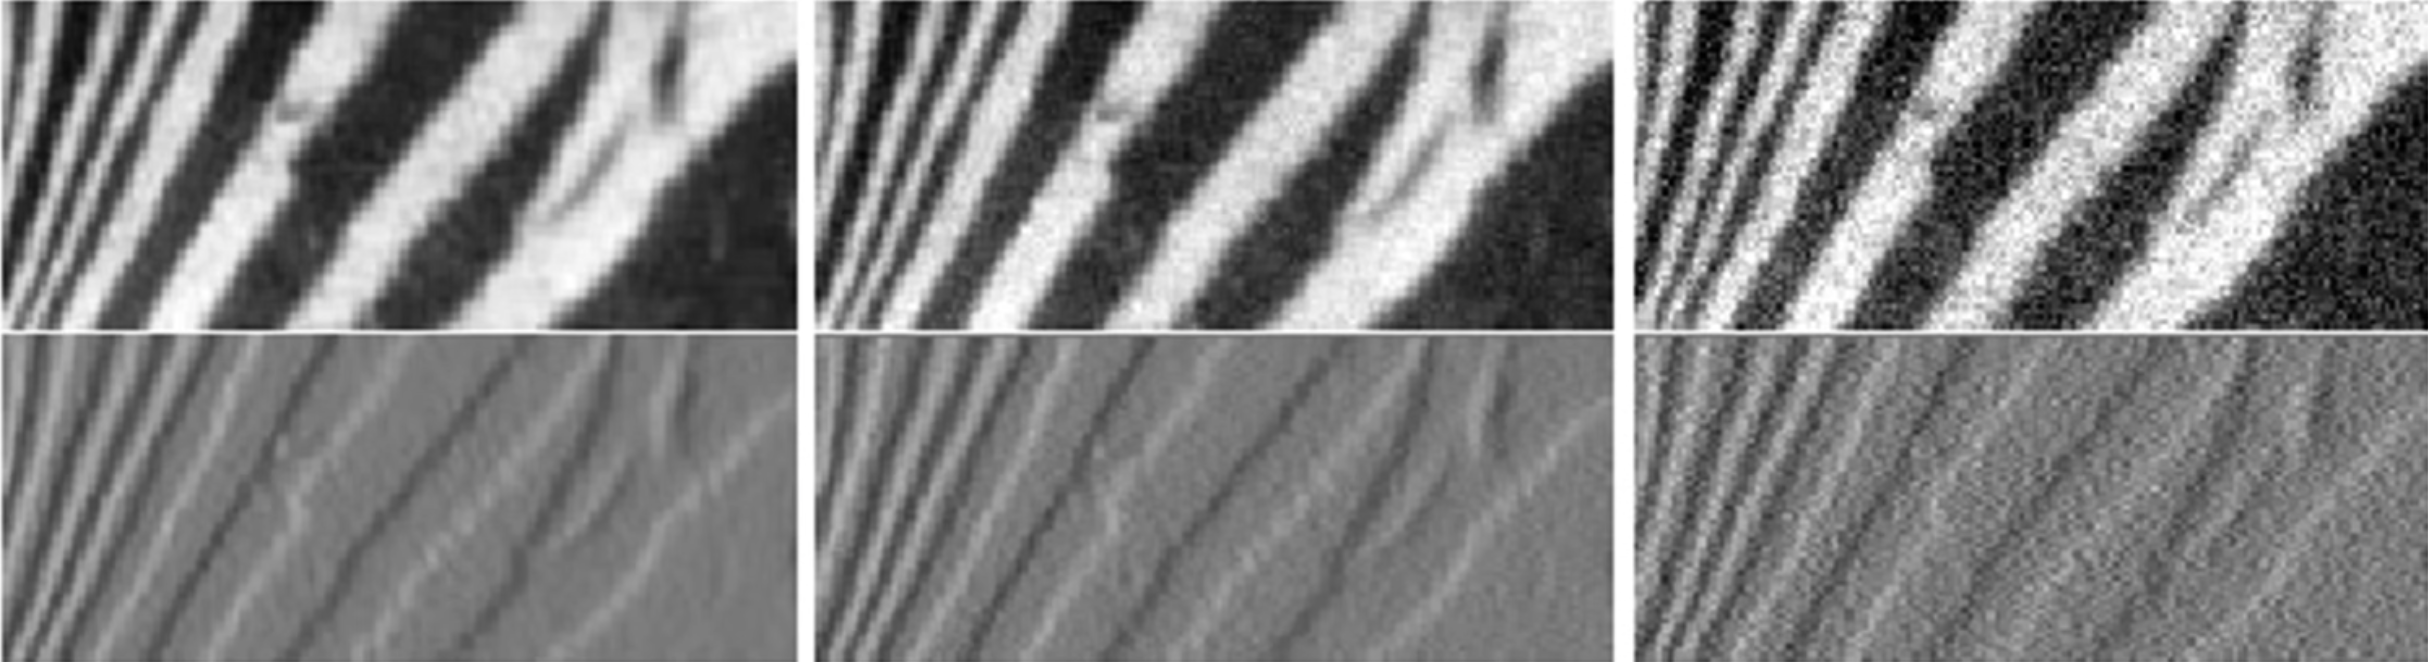
\includegraphics[width=\textwidth]{images/noise_impact}
	\caption{Noise impact on the gradient image}
	\source{\cite{modern-approach}, Figure 8.10}
	\label{fig:noise_impact}
\end{figure}

\subsection{Edge detection in general\cite{digital-image-processing}}
Primary edge detection steps include:
\begin{itemize}
	\item Smoothing derivatives to suppress noise and compute gradient
	\item Threshold to find regions of "significant" gradient
	\item Thinning to get localized edge pixels
	\item Connecting edge pixels
\end{itemize}

\subsection{Canny Edge Detection}
In particular, Canny edge operator consists of following steps\cite{canny-edge}:
\begin{enumerate}
	\item Filtering the image with derivative of Gaussian
	\item Finding the magnitude and the orientation of the gradient
	\item Performing non-maximum suppression: thinning multi-pixel wide ridges (as the edges may have been broadened in step 1.) down to single pixel width
	\item Linking and thresholding (hysteresis). To perform this step two thresholds are defined: low and high. Then it continues as follows:
	\begin{enumerate}
		\item The high threshold is applied to detect strong edge pixels
		\item Strong edge pixels are linked to form strong edges
		\item The low threshold is applied to find weak, but plausible, edge pixels
		\item Strong edges are extended to follow weak edge pixels
	\end{enumerate}
\end{enumerate}

\section{Hough Lines Detection}
\paragraph{Voting}
is a general technique where we let all the features vote for all models that are compatible with it.
\begin{enumerate}
	\item Cycle through features, each casting votes for model parameters.
	\item Look for model parameters that receive a lot of votes.
\end{enumerate}

\paragraph{Hough Line Transform}
is a voting technique that can be used to answer all of the following questions\cite{introduction-to-computer-vision}:
\begin{itemize}
	\item Given points that belong to a line, what is the line?
	\item How many lines are there?
	\item Which points belong to which lines?
\end{itemize}
In order to use Hough Line Transform, the image should be binary. The most common approach is to convert color image to grayscale, then apply edge detection to obtain the edge pixels. This binary image then undergoes Hough transformation that outputs a set of lines that were found. The main idea of this algorithm is as follows:
\begin{enumerate}
	\item Each edge pixel votes for compatible lines
	\item Look for lines that got many votes
\end{enumerate}

\paragraph{Line representations}
Let us now look at the possible representations of a line. The simplest and most widely used one is using Cartesian coordinates (see Figure \ref{fig:line_cartesian}):
\begin{equation}
	y = m x + b
\end{equation}
where $m$ represents the slope and $b$ the intercept with Y-axis.
\begin{figure}[H]
	\centering
	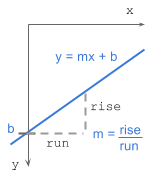
\includegraphics[width=0.3\textwidth]{images/hough_cartesian_equation}
	\caption{Line represented in Cartesian coordinates}
	\source{\cite{hough-lines-python}}
	\label{fig:line_cartesian}
\end{figure}
Other possible representation of a line is in polar coordinates (see Figure \ref{fig:line_polar}):
\begin{equation}
	\rho = x \cos\theta + y \sin\theta
\end{equation}
where $\rho$ represents the perpendicular distance from origin to the line and $\theta$ the angle the perpendicular makes with with the X-axis.
\begin{note}
	The OpenCV implementation of the Hough Lines algorithm returns the $\theta$ with values from range $[0, \pi]$ and allows negative $\rho$.
\end{note}
\begin{figure}[H]
	\centering
	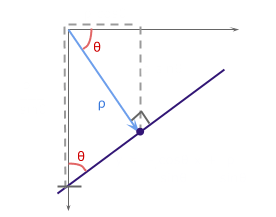
\includegraphics[width=0.3\textwidth]{images/hough_polar}
	\caption{Line represented in polar coordinates}
	\source{\cite{hough-lines-python}}
	\label{fig:line_polar}
\end{figure}

\paragraph{Hough space}
Let us now consider Image Space to be represented in polar coordinates. A line is then represented by some $\rho$ and $\theta$. We can draw such a point in $(\rho, \theta)$ coordinates that will be called \textbf{Hough space}.\cite{hough-lines}
\begin{figure}[H]
	\centering
	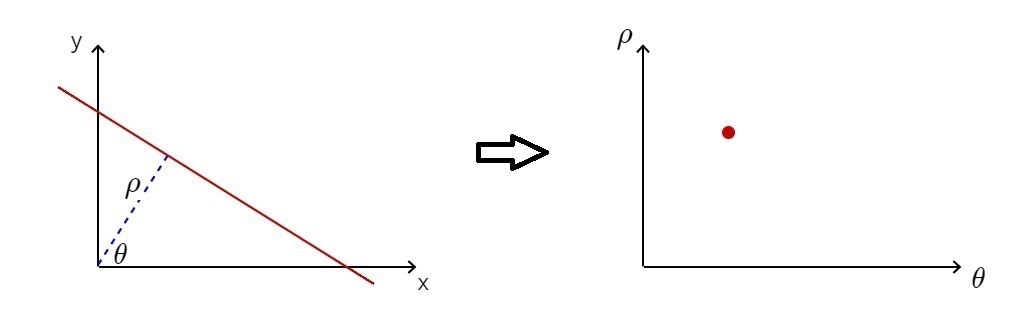
\includegraphics[width=\textwidth]{images/line_to_hough_space}
	\caption{Line represented in Hough space}
	\source{\cite{hough-lines}}
	\label{fig:line_hough_space}
\end{figure}
\begin{figure}[H]
	\centering
	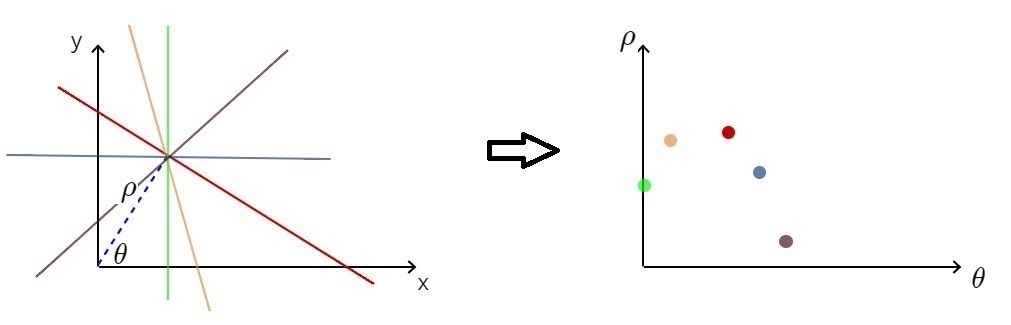
\includegraphics[width=\textwidth]{images/lines_to_hough_space}
	\caption{Bunch of lines with common point represented in Hough space}
	\source{\cite{hough-lines}}
	\label{fig:bunch_of_lines_hough_space}
\end{figure}
It turns out that a point in image space results in a sinusoid in Hough space.
\begin{figure}[H]
	\centering
	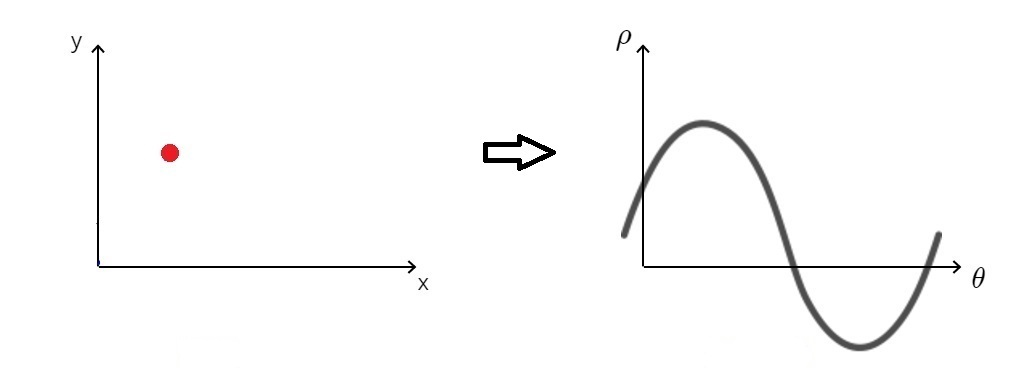
\includegraphics[width=\textwidth]{images/point_to_sinusoid}
	\caption{Point in image space represented as sinusoid in Hough space}
	\source{\cite{hough-lines}}
	\label{fig:point_to_sinusoid}
\end{figure}
\begin{table}[H]
	\centering
	\begin{spacing}{1.5}
	\begin{tabular}{|l|l|}
		\hline
		\textbf{Image space} & \textbf{Hough space} \\ [0.5ex]
		\hline
		Straight line & Point \\ [0.5ex]
		\hline
		Point & Sinusoid \\ [0.5ex]
		\hline
	\end{tabular}
	\end{spacing}
	\caption{Duality between image space and Hough space}
\end{table}
Finally, take a look at points that are forming a line in image space and their corresponding sinusoids in Hough space (Figure \ref{fig:line_detection_in_hough_space}). We can see, that all of the sinusoids intersect at exactly one point that represents the $(\rho, \theta)$ parameters of our line in image space.
\begin{figure}[H]
	\centering
	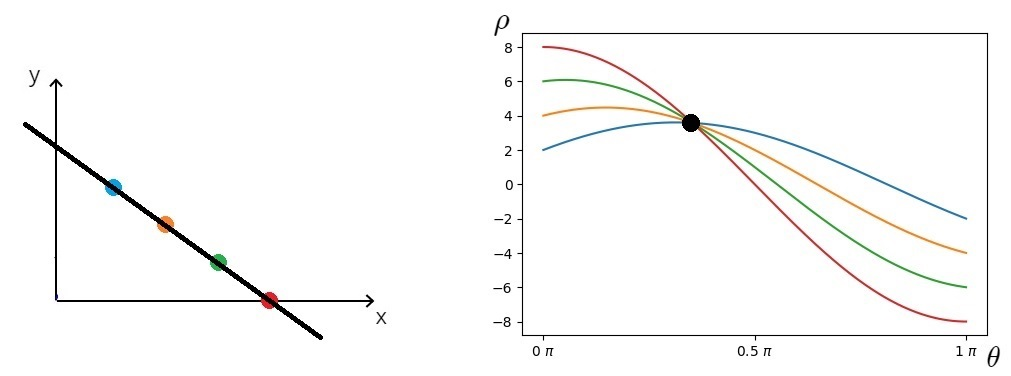
\includegraphics[width=\textwidth]{images/points_to_sinusoids}
	\caption{Detecting a line in Hough space}
	\source{\cite{hough-lines}}
	\label{fig:line_detection_in_hough_space}
\end{figure}

\paragraph{Hough Line Transform}
Let us now look how it all works for actually finding the lines. As mentioned earlier, the algorithm uses a voting technique, so we let each edge pixel to cast its votes. An accumulator (a matrix) is created to hold those votes. Looping over the edge pixels, we generate sinusoidal curves that correspond to this point in Hough space for each $\theta$ in range $[0, \pi]$ given some step ($\delta$). For that value of $\theta$ the corresponding $\rho$ is computed (from the line equation: $\rho = x\cos\theta + y\sin\theta$). Such a $(\theta, \rho)$ pair increments corresponding count of votes in the accumulator matrix. Then next value of $\theta$ is taken and the procedure repeats. This continues up until $\theta$ is equal to $\pi$  and for each of those values votes are "casted". Then next edge pixel is taken and is voting. The procedure ends when no edge pixel is left to vote. Cells from the accumulator matrix that have a lot of votes correspond to lines in image space.

\begin{algorithm}
	\begin{spacing}{1.5}
	\begin{algorithmic}[1]
		\Function{hough\_line\_transform}{$edge\_image$}
			\State Initialize $H[\rho, \theta] = 0$
			\For{$edge\_pixel$ \textbf{in} $edge\_image$}
				\For{$\theta$ \textbf{in} \textbf{range}$(0, 180, \delta)$}
					\State $\rho \gets x\cos\theta + y\sin\theta$
					\State $H[\rho, \theta] += 1$
				\EndFor
			\EndFor
			\State Find value(s) of $(\rho, \theta)$ where $H[\rho, \theta]$ is a local maximum
		\EndFunction
	\end{algorithmic}
	\end{spacing}
	\caption{Hough Line Transform}
\end{algorithm}

\begin{note}
It is worth noting, that the accuracy of this algorithm highly depends on the number of cells in the accumulator matrix. If, for example the step $\delta$ was $45^{\circ}$ we would only have $\{0^{\circ}, 45^{\circ}, 90^{\circ}, 135^{\circ}, 180^{\circ}\}$ as the cells for $\theta$ value. The voting process would then be highly inaccurate. It also cannot be to granular, because this technique depends on relatively high number of votes to be casted in a small region.
\end{note}

Figure \ref{fig:hough-line-transform} shows an edge image that contains two visible lines $(a)$. Applying the Hough Line Transform outputs the results that are visualized on image $(b)$. Sinusoidal curves that correspond to edge pixels are shown. We can observe two very bright spots where a large number of curves intersect. This means that those spots (some $(\rho, \theta)$ pairs) have gained a lot of votes in the accumulator matrix. Hence, they are yield as lines that are marked on the output image $(c)$.

\begin{figure}[H]
     \centering
     \subfloat[Input image]{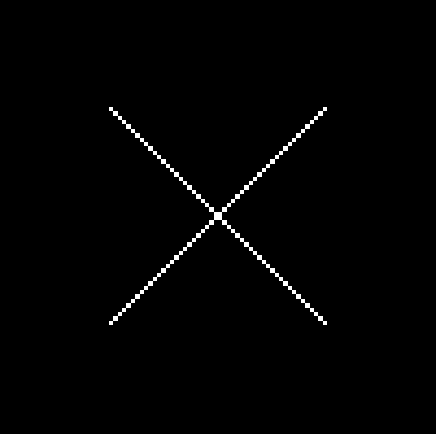
\includegraphics[width=0.3\textwidth]{images/hough_input}}
     \hfill
     \subfloat[Hough Line Transform]{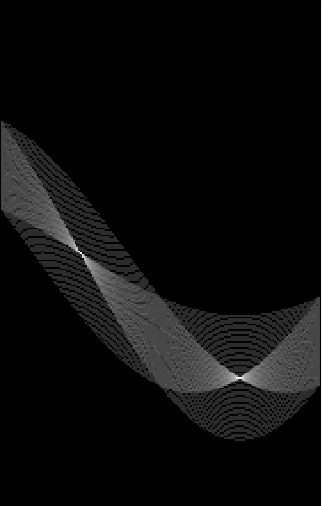
\includegraphics[width=0.3\textwidth]{images/hough_transform}}
     \hfill
     \subfloat[Lines found]{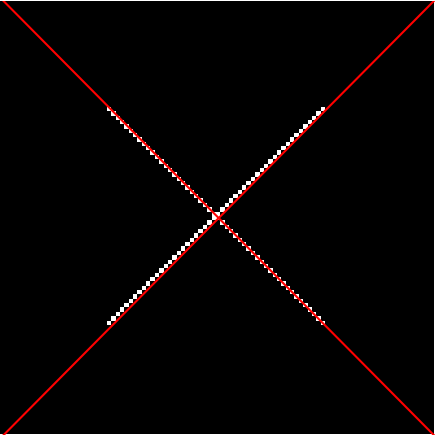
\includegraphics[width=0.3\textwidth]{images/hough_output}}
     \caption{Example of applying Hough Line Transform}
     \source{\url{http://scikit-image.org/docs/0.9.x/auto_examples/plot_line_hough_transform.html}}
     \label{fig:hough-line-transform}
\end{figure}
